\section{Problem Statement}
\label{sec:statement}

In addition to the problem statement given in the caption of
Figure~\ref{fig:problem}, we will also seek to find the path that yields the
shortest distance from the vertex $P$ to the point $T$, which lies in the middle
of the vertices $O$ and $R$.

\begin{figure}[h]
  \centering
  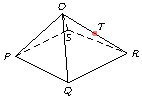
\includegraphics[trim={0 0 0 0cm},clip,width=0.5\textwidth]{./figures/pyramid.pdf}
  \vspace{-8mm}
  \caption{Shown above is a regular square pyramid all of whose sides have
  length of $2\ell$. We seek to find the shortest distance from the vertex $P$
  to the midpoint $T$ of points $O$ and $R$.}
  \label{fig:problem}
\end{figure}

% \begin{enumerate}
%   \setlength\itemsep{0em}
%   \item Find the map $f: \mathbb{R}_+^2 \rightarrow \mathbb{R}_+^2$ that takes
%           the side lengths of the rectangle $(w,h)$ to $(r, \abs{XY})$, the
%           radius of one of the circles and the length of the line segment $XY$.
%   \item Find the inverse $f^{-1}$ of $f$, that takes $(r, \abs{XY})$ to $(w,h)$.
% \end{enumerate}

